%!TEX root = ../../main.tex
% ============================================================
% 统计图表 / 频数直方图
% 本文件由 main.tex 通过 \input 引入，请勿单独编译
% 重构日期: 2026-04-11
% ============================================================

\subsection{解答：身体素质测试频数分布与直方图}

\vspace{0.6cm}

\textbf{例 八年级(1)班进行了一次身体素质测试，每名学生的成绩如下（单位：分）：\\
$66, 83, 92, 54, 68, 82, 63, 63, 95, 73, 71, 89, 83, 64, 75,$ \\
$85, 79, 96, 68, 64, 83, 91, 70, 70, 85, 83, 89, 95, 86, 84,$ \\
$63, 71, 85, 86, 71, 82, 94, 54, 68, 79, 51, 82, 73, 59, 85.$}

\vspace{0.4cm}

\textbf{解：}

\textbf{（1）整理数据并完善表格：} \\
数据总个数：$3$ 行 $\times 15$ 列 $= 45$ 名学生。逐个区间进行排查统计：
\begin{itemize}
  \item \textbf{$\boldsymbol{49.5 \leqslant x < 59.5}$：} 包含 $54, 54, 51, 59$，频数为 $\boldsymbol{4}$，划记为“\zhengIV{}”。
  \item \textbf{$\boldsymbol{59.5 \leqslant x < 69.5}$：} 包含 $66, 68, 63, 63, 64, 68, 64, 63, 68$，频数为 $\boldsymbol{9}$，划记为“\zhengV{} \zhengIV{}”。
  \item \textbf{$\boldsymbol{69.5 \leqslant x < 79.5}$：} 包含 $73, 71, 75, 79, 70, 70, 71, 71, 79, 73$，频数为 $\boldsymbol{10}$，与原题一致“\zhengV{} \zhengV{}”。
  \item \textbf{$\boldsymbol{79.5 \leqslant x < 89.5}$：} 包含 $83, 82, 89, 83, 85, 83, 85, 83, 89, 86, 84, 85, 86, 82, 82, 85$，频数为 $\boldsymbol{16}$，划记为“\zhengV{} \zhengV{} \zhengV{} \zhengI{}”。
  \item \textbf{$\boldsymbol{89.5 \leqslant x < 99.5}$：} 包含 $92, 95, 96, 91, 95, 94$，频数为 $\boldsymbol{6}$，划记为“\zhengV{} \zhengI{}”。
\end{itemize}

填写表格（首列恢复灰底设计，红字为补充填写数据）：

\vspace{0.4cm}

\begin{center}
\renewcommand{\arraystretch}{1.6}
\resizebox{\textwidth}{!}{%
\begin{tabular}{|>{\columncolor{gray!15}\centering\arraybackslash}p{2.2cm}|>{\centering\arraybackslash}p{3cm}|>{\centering\arraybackslash}p{3cm}|>{\centering\arraybackslash}p{3cm}|>{\centering\arraybackslash}p{3cm}|>{\centering\arraybackslash}p{3cm}|}
\hline
成绩 $x$/分 & $49.5 \leqslant x < 59.5$ & $59.5 \leqslant x < 69.5$ & $69.5 \leqslant x < 79.5$ & $79.5 \leqslant x < 89.5$ & $89.5 \leqslant x < 99.5$ \\
\hline
频数记录 & \textbf{\textcolor{red!70!black}{\zhengIV{}}} & \textbf{\textcolor{red!70!black}{\zhengV{} \quad \zhengIV{}}} & \textbf{\zhengV{} \quad \zhengV{}} & \textbf{\textcolor{red!70!black}{\zhengV{}~\zhengV{}~\zhengV{}~\zhengI{}}} & \textbf{\textcolor{red!70!black}{\zhengV{} \quad \zhengI{}}} \\
\hline
频 \quad 数 & \textbf{\textcolor{red!70!black}{$4$}} & \textbf{\textcolor{red!70!black}{$9$}} & \textbf{\textcolor{red!70!black}{$10$}} & \textbf{\textcolor{red!70!black}{$16$}} & \textbf{\textcolor{red!70!black}{$6$}} \\
\hline
\end{tabular}%
}
\end{center}


\vspace{0.8cm}

\textbf{（2）根据统计表绘制频数分布直方图。}

\vspace{0.4cm}
\begin{center}
\begin{tikzpicture}[>=Stealth, x=1.8cm, y=0.35cm]

  % Y轴及刻度网格
  \draw[->, line width=0.8pt] (0, 0) -- (0, 18.8) node[above] {频数};
  \foreach \y in {2,4,...,18} {
    \draw[line width=0.8pt] (0, \y) -- (-0.08, \y) node[left, font=\footnotesize] {\y};
    \draw[gray!50, dashed, line width=0.5pt] (0, \y) -- (6.5, \y); % 横向辅助网格线
  }
  \node[left, font=\footnotesize] at (0, 0) {$0$};

  % X轴及截断曲线
  \draw[line width=0.8pt] (0, 0) -- (0.35, 0) -- (0.42, 0.8) -- (0.58, -0.8) -- (0.65, 0);
  \draw[->, line width=0.8pt] (0.65, 0) -- (6.8, 0) node[right] {成绩/分};

  % X轴刻度：每一个条形的边界
  \foreach \x/\label in {1/49.5, 2/59.5, 3/69.5, 4/79.5, 5/89.5, 6/99.5} {
    \draw[line width=0.8pt] (\x, 0) -- (\x, -0.3) node[below, font=\small] {\label};
  }

  % 直方图矩形体及顶端频数标记
  % 第1组 [49.5, 59.5] 频数 4
  \draw[fill=gray!15, line width=0.8pt] (1, 0) rectangle (2, 4);
  \node[above, font=\small\bfseries, text=red!70!black] at (1.5, 4) {4};

  % 第2组 [59.5, 69.5] 频数 9
  \draw[fill=gray!15, line width=0.8pt] (2, 0) rectangle (3, 9);
  \node[above, font=\small\bfseries, text=red!70!black] at (2.5, 9) {9};

  % 第3组 [69.5, 79.5] 频数 10
  \draw[fill=gray!15, line width=0.8pt] (3, 0) rectangle (4, 10);
  \node[above, font=\small\bfseries, text=red!70!black] at (3.5, 10) {10};

  % 第4组 [79.5, 89.5] 频数 16
  \draw[fill=gray!15, line width=0.8pt] (4, 0) rectangle (5, 16);
  \node[above, font=\small\bfseries, text=red!70!black] at (4.5, 16) {16};

  % 第5组 [89.5, 99.5] 频数 6
  \draw[fill=gray!15, line width=0.8pt] (5, 0) rectangle (6, 6);
  \node[above, font=\small\bfseries, text=red!70!black] at (5.5, 6) {6};

\end{tikzpicture}
\end{center}

\vspace{0.6cm}

{\small\color{blue!70!black}
\textbf{制图（直方图）与绘表原理分析：}\\
\textbf{1. 异形行标题底色控制：} 根据题目风格，表头在最左侧的一列，调用 \texttt{>\{\textbackslash columncolor\{gray!15\}\textbackslash centering\textbackslash arraybackslash\}p\{\dots\}} 单独对此列进行纯灰着色，实现了“成绩/频数记录/频数”单元格列的灰阶渲染，匹配原图的特征。\\
\textbf{2. 截断坐标标记构造：} 直方图数据横轴非零出发，我在 $X=0.5$ 区域用 \texttt{TikZ} 手动控制路径 \texttt{(0,0) -- (0.35,0) -- (0.42,0.8) -- (0.58,-0.8) -- (0.65,0)} 绘制了标准统计图特有的锯齿断崖表示省略非统计区间。\\
\textbf{3. 自适应坐标系缩放：} 为了避免直方图在纸面上过长或过扁，定义了 \texttt{x=1.8cm, y=0.35cm} 这一套自适应缩放机制；让最大频数 $16$ 的柱高保持在约 $5.6\text{cm}$，让横轴的带小数文本互不穿插。所有背景附加 \texttt{gray!50} 虚线作为对齐网格，柱体填充 \texttt{gray!15} 避免纯白过虚。
}

%% ==============================
%% 第5题：雷达测速频数分布与直方图
%% ==============================
\newpage

\newpage

\subsection{解答：雷达测速频数分布与直方图}

\vspace{0.6cm}

\textbf{2. 将某测速区雷达监测到的一组汽车的速度（单位：km/h）数据整理，得到频数分布表。}

\vspace{0.4cm}

\textbf{解：}

\textbf{（1）请把表中的数据填写完整。} \\
根据第一组已知数据（速度 $30 < x \leqslant 40$），该组频数为 $14$，频率为 $0.07$：
\begin{itemize}
  \item \textbf{样本总数（总计）：} $14 \div 0.07 = \boldsymbol{200}$（辆）。因此最后一行“总计”的频数为 $\boldsymbol{200}$。
  \item \textbf{$40 < x \leqslant 50$ 组：} 频率 $= 50 \div 200 = \boldsymbol{0.25}$。
  \item \textbf{$50 < x \leqslant 60$ 组：} 频数 $= 200 \times 0.48 = \boldsymbol{96}$。
  \item \textbf{$60 < x \leqslant 70$ 组：} 频数 $= 200 - 14 - 50 - 96 - 18 = \boldsymbol{22}$；对应频率 $= 22 \div 200 = \boldsymbol{0.11}$。
\end{itemize}

填补完整的图表如下（红字为补充填写的数据）：

\vspace{0.4cm}
\begin{center}
\renewcommand{\arraystretch}{1.6}
\begin{tabular}{|>{\centering\arraybackslash}p{4.5cm}|>{\centering\arraybackslash}p{3cm}|>{\centering\arraybackslash}p{3cm}|}
\hline
\cellcolor{gray!15} 速度 $x$/(km/h) & \cellcolor{gray!15} 频 \quad 数 & \cellcolor{gray!15} 频 \quad 率 \\
\hline
$30 < x \leqslant 40$ & $14$ & $0.07$ \\
\hline
$40 < x \leqslant 50$ & $50$ & \textbf{\textcolor{red!70!black}{$0.25$}} \\
\hline
$50 < x \leqslant 60$ & \textbf{\textcolor{red!70!black}{$96$}} & $0.48$ \\
\hline
$60 < x \leqslant 70$ & \textbf{\textcolor{red!70!black}{$22$}} & \textbf{\textcolor{red!70!black}{$0.11$}} \\
\hline
$70 < x \leqslant 80$ & $18$ & $0.09$ \\
\hline
总计 & \textbf{\textcolor{red!70!black}{$200$}} & $1$ \\
\hline
\end{tabular}
\end{center}

\vspace{0.6cm}

\textbf{（2）此次调查采用了什么调查方式？}

\vspace{0.2cm}
\textbf{答：}采用了\textbf{抽样调查}的方式。（雷达监测到的是该路段“一组”汽车的速度，代表从该测速区所有车流中抽取的一个样本进行统计分析）。

\vspace{0.6cm}

\textbf{（3）绘制频数分布直方图。}

\vspace{0.4cm}
\begin{center}
\begin{tikzpicture}[>=Stealth, x=1.8cm, y=0.06cm]

  % Y轴及刻度网格 (最大频数为 96，故设置图表界限最大刻度为 100，每 20 一档)
  \draw[->, line width=0.8pt] (0, 0) -- (0, 110) node[above] {频数};
  \foreach \y in {20, 40, 60, 80, 100} {
    \draw[line width=0.8pt] (0, \y) -- (-0.08, \y) node[left, font=\footnotesize] {\y};
    % 横向平行辅助数据网格对齐线 (灰度偏淡化显示)
    \draw[gray!50, dashed, line width=0.5pt] (0, \y) -- (6.5, \y); 
  }
  \node[left, font=\footnotesize] at (0, 0) {$0$};

  % X轴及截断跳跃曲线标记 (起点由于为30不收敛为0)
  \draw[line width=0.8pt] (0, 0) -- (0.35, 0) -- (0.42, 5) -- (0.58, -5) -- (0.65, 0);
  \draw[->, line width=0.8pt] (0.65, 0) -- (6.8, 0) node[right] {速度};

  % X轴区间刻度标记：标识每一个柱状条形的物理边界区
  \foreach \x/\label in {1/30, 2/40, 3/50, 4/60, 5/70, 6/80} {
    \draw[line width=0.8pt] (\x, 0) -- (\x, -1.8) node[below, font=\small] {\label};
  }

  % 逐次渲染直方图内部实体及顶部的红字频数标签
  % 第1组：[30, 40] 对应频数 14
  \draw[fill=gray!15, line width=0.8pt] (1, 0) rectangle (2, 14);
  \node[above, font=\small\bfseries, text=red!70!black] at (1.5, 14) {14};

  % 第2组：[40, 50] 对应频数 50
  \draw[fill=gray!15, line width=0.8pt] (2, 0) rectangle (3, 50);
  \node[above, font=\small\bfseries, text=red!70!black] at (2.5, 50) {50};

  % 第3组：[50, 60] 对应频数 96
  \draw[fill=gray!15, line width=0.8pt] (3, 0) rectangle (4, 96);
  \node[above, font=\small\bfseries, text=red!70!black] at (3.5, 96) {96};

  % 第4组：[60, 70] 对应频数 22
  \draw[fill=gray!15, line width=0.8pt] (4, 0) rectangle (5, 22);
  \node[above, font=\small\bfseries, text=red!70!black] at (4.5, 22) {22};

  % 第5组：[70, 80] 对应频数 18
  \draw[fill=gray!15, line width=0.8pt] (5, 0) rectangle (6, 18);
  \node[above, font=\small\bfseries, text=red!70!black] at (5.5, 18) {18};

\end{tikzpicture}
\end{center}

\vspace{0.6cm}

\textbf{（4）如果此的汽车速度超过 $60\text{ km/h}$ 即为违章，那么违章车辆共有多少辆？}

\vspace{0.2cm}

由频数分布数据表可知，速度严格超过 $60\text{ km/h}$ 的车辆分布在“$60 < x \leqslant 70$”和“$70 < x \leqslant 80$”这两个数据组内。\\
因此此的违章车辆统计总共为：$22 + 18 = \boldsymbol{40}$（辆）。

\textbf{答：} 违章车辆共有 $40$ 辆。

\vspace{0.6cm}

{\small\color{blue!70!black}
\textbf{制表与绘图（直方图）原理步骤分析：}\\
\textbf{1. 大尺度直方图系统的坐标缩放换算：} 本统计体量最大频数已达到了 $96$ 的量级高度，此时如果延续直方图普通的 $1:1$ 或者浅倍数呈现 $Y$ 轴将会直接炸毁排版引发越界。因此在此次算法里，我重新定义了全局竖向的极缩比例尺 \texttt{y=0.06cm}；这表明 $100$ 单位的峰值雷达频数在纸面上会安全折算为刚好 $6\text{cm}$ 左右的安全物理高度；配合内部对齐辅助虚格底纹不仅不显突兀反而让整体画风专业清爽。\\
\textbf{2. 截断标记高度换算的曲线补偿逻辑：} 由于前端数据的非零首发特性，我们需要加入代表性截断标记符号。因为此刻承受了十多倍强烈纵切缩放比，如果不人为干涉会导致截断跳跃波浪呈现成直线看不见。所以这里对波峰高度参数也进行了修正化放大（例如其中的折线点 \texttt{(0.42, 5)} 实际在图纸上通过极缩抵消转化出的物理上扬高度 $= 5 \times 0.06 = 0.3\text{cm}$），一劳永逸解决了超窄比例下起点截断标识消失失效的常见绘制问题。\\
\textbf{3. 表头灰底独立设计法：} 原题目中的首行展现了明暗的经典矩阵排版风格隔离功能；我的代码在 \texttt{tabular} 定义的第一行内主动为每一个单元格均调用了 \texttt{\textbackslash cellcolor\{gray!15\}} 提供染色，高保真还原了题干的原滋原味灰底清爽样貌。
}

%% ==============================
%% 第6题：跳绳成绩频数分布与直方图
%% ==============================
\newpage

\newpage

\subsection{解答：跳绳成绩频数分布与直方图}

\vspace{0.6cm}

\textbf{4. 体育老师统计了全班学生 $60\text{ s}$ 跳绳的次数，并列出下面的频数分布表：}

\vspace{0.4cm}
% 原表格重现
\begin{center}
\renewcommand{\arraystretch}{1.6}
\resizebox{\textwidth}{!}{%
\begin{tabular}{|>{\columncolor{gray!15}\centering\arraybackslash}p{1.5cm}|c|c|c|c|c|c|c|}
%\begin{tabular}{|>{\columncolor{gray!15}\centering\arraybackslash}p{1.5cm}|>{\centering\arraybackslash}p{2.2cm}|>{\centering\arraybackslash}p{2.4cm}|>{\centering\arraybackslash}p{2.5cm}|>{\centering\arraybackslash}p{2.5cm}|>{\centering\arraybackslash}p{2.5cm}|>{\centering\arraybackslash}p{2.5cm}|>{\centering\arraybackslash}p{2.5cm}|}
\hline
\makecell{次数\\$x$} & $60 \leqslant x < 80$ & $80 \leqslant x < 100$ & $100 \leqslant x < 120$ & $120 \leqslant x < 140$ & $140 \leqslant x < 160$ & $160 \leqslant x < 180$ & $180 \leqslant x < 200$ \\
\hline
频数 & $2$ & $4$ & $21$ & $13$ & $8$ & $4$ & $1$ \\
\hline
\end{tabular}%
}
\end{center}

\vspace{0.4cm}

\textbf{解：}

\textbf{（1）全班有多少名学生？} \\
将所有频数组相加得到班级总人数：
$$2 + 4 + 21 + 13 + 8 + 4 + 1 = \boldsymbol{53}\text{（名）}$$
\textbf{答：} 全班共有 $53$ 名学生。

\vspace{0.4cm}

\textbf{（2）组距是多少？组数是多少？} \\
组距 $=$ 每个区间的上限 $-$ 下限 $= 80 - 60 = \boldsymbol{20}$。\\
组数 $=$ 频数分布表内划分的数据区间总数 $= \boldsymbol{7}$（组）。\\
\textbf{答：} 组距是 $20$，组数是 $7$。

\vspace{0.4cm}

\textbf{（3）跳绳次数 $x$ 在 $100 \leqslant x < 140$ 范围内的学生有多少名？占全班学生的百分之几？} \\
该范围包含了 $100 \leqslant x < 120$ 与 $120 \leqslant x < 140$ 两个区间：\\
学生人数 $= 21 + 13 = \boldsymbol{34}\text{（名）}$。\\
所占百分比为：$\frac{34}{53} \times 100\% \approx \boldsymbol{64.15\%}$。\\
\textbf{答：} 该范围内的学生有 $34$ 名，约占全班学生的 $64.15\%$。

\vspace{0.4cm}

\textbf{（4）画出适当的统计图表示上面的信息。} \\
（这里选择最为直观的\textbf{频数分布直方图}进行绘制）：

\vspace{0.4cm}
\begin{center}
\begin{tikzpicture}[>=Stealth, x=1.5cm, y=0.25cm]

  % Y轴及网格线 (最大频数为 21，设置Y轴边界为 25，步长为 5)
  \draw[->, line width=0.8pt] (0, 0) -- (0, 25) node[above] {频数};
  \foreach \y in {5, 10, 15, 20} {
    \draw[line width=0.8pt] (0, \y) -- (-0.08, \y) node[left, font=\footnotesize] {\y};
    \draw[gray!50, dashed, line width=0.5pt] (0, \y) -- (8.5, \y); % 横向辅助对齐网格
  }
  \node[left, font=\footnotesize] at (0, 0) {$0$};

  % X轴及截断跳跃曲线 (起点数据为60，故折叠波浪省略0至60的空白区间)
  \draw[line width=0.8pt] (0, 0) -- (0.35, 0) -- (0.42, 1.2) -- (0.58, -1.2) -- (0.65, 0);
  \draw[->, line width=0.8pt] (0.65, 0) -- (8.8, 0) node[right] {次数};

  % X轴刻度边界
  \foreach \x/\label in {1/60, 2/80, 3/100, 4/120, 5/140, 6/160, 7/180, 8/200} {
    \draw[line width=0.8pt] (\x, 0) -- (\x, -0.6) node[below, font=\small] {\label};
  }

  % 逐组绘制直方图柱状体及顶端频数标记
  % 第1组
  \draw[fill=gray!15, line width=0.8pt] (1, 0) rectangle (2, 2);
  \node[above, font=\small\bfseries, text=red!70!black] at (1.5, 2) {2};

  % 第2组
  \draw[fill=gray!15, line width=0.8pt] (2, 0) rectangle (3, 4);
  \node[above, font=\small\bfseries, text=red!70!black] at (2.5, 4) {4};

  % 第3组
  \draw[fill=gray!15, line width=0.8pt] (3, 0) rectangle (4, 21);
  \node[above, font=\small\bfseries, text=red!70!black] at (3.5, 21) {21};

  % 第4组
  \draw[fill=gray!15, line width=0.8pt] (4, 0) rectangle (5, 13);
  \node[above, font=\small\bfseries, text=red!70!black] at (4.5, 13) {13};

  % 第5组
  \draw[fill=gray!15, line width=0.8pt] (5, 0) rectangle (6, 8);
  \node[above, font=\small\bfseries, text=red!70!black] at (5.5, 8) {8};

  % 第6组
  \draw[fill=gray!15, line width=0.8pt] (6, 0) rectangle (7, 4);
  \node[above, font=\small\bfseries, text=red!70!black] at (6.5, 4) {4};

  % 第7组
  \draw[fill=gray!15, line width=0.8pt] (7, 0) rectangle (8, 1);
  \node[above, font=\small\bfseries, text=red!70!black] at (7.5, 1) {1};

\end{tikzpicture}
\end{center}

\vspace{0.4cm}

\textbf{（5）你怎样评价这个班的跳绳成绩？} \\
\textbf{答：} 这个班跳绳成绩\textbf{整体水平较好}。主要理由如下：全班绝大多数学生的跳绳次数集中在 $100$ 次以上（共有 $21+13+8+4+1 = 47$ 人），这说明达标率很高；且最多人数集中在 $100 \sim 120$ 次之间（$21$人）。只有极少数学生（$6$人）成绩低于 $100$ 次，体现了该班体育素质整体偏优异且分布均匀集中。

\vspace{0.6cm}

{\small\color{blue!70!black}
\textbf{制图（直方图）物理逻辑与原理步骤分析：}\\
\textbf{1. 异形长表的版界缩放控制：} 本题给出的原数据表宽达惊人的 $8$ 列长横向并排尺寸。如果在排版中稍不注意很容易造成右侧超界截断成残缺。因此我预先便套用了超强宏包渲染容器 \texttt{\textbackslash resizebox\{\textbackslash textwidth\}\{!\}\{\dots\}} 进行外壳包裹，使原本长表格结构被迫同比平滑缩限在一个合法的 \texttt{\textbackslash textwidth} 物理底纸安全线范围内。\\
\textbf{2. 坐标刻崖断点设计分析：} 直方图起跳点跨度为极大的 $60$；为此我利用 \texttt{TikZ} 点阵路线 \texttt{(0,0) -- (0.35,0) -- (0.42, 1.2) -- (0.58, -1.2) -- (0.65, 0)} 在毫厘之间凭空生成压缩跳跃折叠符号，使得视觉与学科数据的映射更加匹配且学术呈现严谨。\\
\textbf{3. 自下而上的刻度高度控制法则：} 考虑到最高柱峰数值为 $21$，配置 $y=0.25\text{cm}$ 物理比例缩放；让它以最优解恰好止步在了不足 $6\text{cm}$ 的打印物理表现范围内。保证了原先题意数据的学术感和辨识度，且与灰白柱身加红字构成了非常优质的印刷观感。
}

%% ==============================
%% 第7题：果园结果数量频数分布与直方图
%% ==============================
\newpage

\newpage

\subsection{解答：果园结果数量频数分布与直方图}

\vspace{0.6cm}

\textbf{5. 某果园有 $40$ 棵苹果树，2025 年每棵苹果树的结果数量（单位：个）如下：\\
$28, 62, 54, 29, 32, 47, 75, 55, 43, 36, 46, 54, 39, 32, 64, 61, 59, 67, 56, 45,$ \\
$49, 36, 39, 52, 65, 48, 58, 59, 64, 67, 54, 57, 68, 54, 71, 59, 47, 58, 52, 52.$ \\
请按组距为 10 将数据分组，列出频数分布表，绘制频数分布直方图，分析数据分布的情况。}

\vspace{0.4cm}

\textbf{解：}

\textbf{（1）按组距将数据分组，列出频数分布表} \\
由于给出的结果数量数据中，最小值为 $28$，最大值为 $75$，要求组距为 $10$；故我们划分下界从最近的整十数 $20$ 起步，以 $10$ 为间距分为 $6$ 组进行扫掠统计：
\begin{itemize}
  \item \textbf{$\boldsymbol{20 \leqslant x < 30}$：} 包含 $28, 29$，频数为 $\boldsymbol{2}$。
  \item \textbf{$\boldsymbol{30 \leqslant x < 40}$：} 包含 $32, 36, 39, 32, 36, 39$，频数为 $\boldsymbol{6}$。
  \item \textbf{$\boldsymbol{40 \leqslant x < 50}$：} 包含 $47, 43, 46, 45, 49, 48, 47$，频数为 $\boldsymbol{7}$。
  \item \textbf{$\boldsymbol{50 \leqslant x < 60}$：} 包含 $54, 55, 54, 59, 56, 52, 58, 59, 54, 57, 54, 59, 58, 52, 52$，频数为 $\boldsymbol{15}$。
  \item \textbf{$\boldsymbol{60 \leqslant x < 70}$：} 包含 $62, 64, 61, 67, 65, 64, 67, 68$，频数为 $\boldsymbol{8}$。
  \item \textbf{$\boldsymbol{70 \leqslant x < 80}$：} 包含 $75, 71$，频数为 $\boldsymbol{2}$。
\end{itemize}

填写如下的频数分布表：

\vspace{0.4cm}
\begin{center}
\renewcommand{\arraystretch}{1.6}
\resizebox{\textwidth}{!}{%
\begin{tabular}{|>{\columncolor{gray!15}\centering\arraybackslash}p{2.5cm}|c|c|c|c|c|c|}
\hline
\makecell{结果数量 \\$x$/个} & $20 \leqslant x < 30$ & $30 \leqslant x < 40$ & $40 \leqslant x < 50$ & $50 \leqslant x < 60$ & $60 \leqslant x < 70$ & $70 \leqslant x < 80$ \\
\hline
频数记录 & \textbf{\textcolor{red!70!black}{\zhengII{}}} & \textbf{\textcolor{red!70!black}{\zhengV{} \quad \zhengI{}}} & \textbf{\textcolor{red!70!black}{\zhengV{} \quad \zhengII{}}} & \textbf{\textcolor{red!70!black}{\zhengV{}~\zhengV{}~\zhengV{}}} & \textbf{\textcolor{red!70!black}{\zhengV{} \quad \zhengIII{}}} & \textbf{\textcolor{red!70!black}{\zhengII{}}} \\
\hline
频 \quad 数 & $\boldsymbol{2}$ & $\boldsymbol{6}$ & $\boldsymbol{7}$ & $\boldsymbol{15}$ & $\boldsymbol{8}$ & $\boldsymbol{2}$ \\
\hline
\end{tabular}%
}
\end{center}

\vspace{0.6cm}

\textbf{（2）绘制频数分布直方图}

\vspace{0.4cm}
\begin{center}
\begin{tikzpicture}[>=Stealth, x=1.6cm, y=0.35cm]

  % Y轴及网格线 (最大频数为 15，设置Y轴边界为 17，步长为 2)
  \draw[->, line width=0.8pt] (0, 0) -- (0, 18) node[above] {频数};
  \foreach \y in {2, 4, 6, 8, 10, 12, 14, 16} {
    \draw[line width=0.8pt] (0, \y) -- (-0.08, \y) node[left, font=\footnotesize] {\y};
    \draw[gray!50, dashed, line width=0.5pt] (0, \y) -- (7.5, \y); % 横向辅助对齐网格
  }
  \node[left, font=\footnotesize] at (0, 0) {$0$};

  % X轴及截断跳跃曲线 (起点数据为20)
  \draw[line width=0.8pt] (0, 0) -- (0.35, 0) -- (0.42, 0.8) -- (0.58, -0.8) -- (0.65, 0);
  \draw[->, line width=0.8pt] (0.65, 0) -- (7.8, 0) node[right] {结果数量/个};

  % X轴刻度边界
  \foreach \x/\label in {1/20, 2/30, 3/40, 4/50, 5/60, 6/70, 7/80} {
    \draw[line width=0.8pt] (\x, 0) -- (\x, -0.4) node[below, font=\small] {\label};
  }

  % 逐组绘制直方图柱状体及顶端频数标记
  % 第1组 [20, 30)
  \draw[fill=gray!15, line width=0.8pt] (1, 0) rectangle (2, 2);
  \node[above, font=\small\bfseries, text=red!70!black] at (1.5, 2) {2};

  % 第2组 [30, 40)
  \draw[fill=gray!15, line width=0.8pt] (2, 0) rectangle (3, 6);
  \node[above, font=\small\bfseries, text=red!70!black] at (2.5, 6) {6};

  % 第3组 [40, 50)
  \draw[fill=gray!15, line width=0.8pt] (3, 0) rectangle (4, 7);
  \node[above, font=\small\bfseries, text=red!70!black] at (3.5, 7) {7};

  % 第4组 [50, 60)
  \draw[fill=gray!15, line width=0.8pt] (4, 0) rectangle (5, 15);
  \node[above, font=\small\bfseries, text=red!70!black] at (4.5, 15) {15};

  % 第5组 [60, 70)
  \draw[fill=gray!15, line width=0.8pt] (5, 0) rectangle (6, 8);
  \node[above, font=\small\bfseries, text=red!70!black] at (5.5, 8) {8};

  % 第6组 [70, 80)
  \draw[fill=gray!15, line width=0.8pt] (6, 0) rectangle (7, 2);
  \node[above, font=\small\bfseries, text=red!70!black] at (6.5, 2) {2};

\end{tikzpicture}
\end{center}

\vspace{0.6cm}

\textbf{（3）分析数据分布的情况} \\
\textbf{答：} 通过频数分布表和直方图可以得出明显的分层结论：
\begin{enumerate}
    \item 总体呈现\textbf{“中间多，两端少”}的正态分布趋势，单峰特征显著，数据集中倾向明显。
    \item 结果数量分布最密集的区间在 $50 \leqslant x < 60$，共有 $15$ 棵树，占总数 $40$ 棵的 $37.5\%$。
    \item 绝大部分该果园的苹果树产量集中在了 $40 \sim 70$ 个果子的范围之内（包含 $7 + 15 + 8 = 30$ 棵，占比高达 $75\%$），这就说明果园的挂果稳定，质量表现可控；极少数树木产果显著较少或产量极高突变，只属个例。
\end{enumerate}

\vspace{0.6cm}

{\small\color{blue!70!black}
\textbf{制图（直方图）物理逻辑与原理步骤分析：}\\
\textbf{1. 柔性矩阵表格自适应（新特性）：} 我吸收了您的修改优化灵感，表主体通过 \texttt{>\{\dots\}p\{2.5cm\}|c|c|c|c|c|c|} 重构代码，既死死锁住了首列宽的溢出隐患，又彻底解放了频数分布列——全交由 \texttt{c} 标签给 Latex 底层编译器自行撑开；辅以外围的 \texttt{\textbackslash resizebox} 保护墙，表体结构展现出史无前例的健壮度！\\
\textbf{2. 梳理原点盲区：} 直方图跳跃范围设定在 $0 \sim 20$ 的非统计真空盲区，我们引入手写断崖波浪号并针对性微增 $Y$ 因子高度消除其缩放失真，使得整个第一数据轴 $20$ 左方非常干净合规。\\
\textbf{3. 自下而上的网格间距步长切分：} 检测到全表频数极值为 $15$，定义了 $Y$ 轴以“步长为 $2$”跨度递进生长直至溢顶至 \texttt{Y=18}，构建出横穿每个立柱的背景辅助定位虚线条，图纸科研质感剧增。
}

%% ==============================
%% 例题：抽样调查与身高频数分布
%% ==============================
\newpage

\newpage

\subsection{解答：抽样调查与身高频数分布}

\vspace{0.6cm}

\textbf{例 为了制定某市七、八、九年级男生校服的生产计划，有关部门准备对这三个年级抽取 $180$ 名男生的身高做调查。现有三种调查方案：\\
① 测量该市少年体校中这三个年级的 $180$ 名男子篮球、排球队员的身高；\\
② 查阅有关这三个年级 $180$ 名男生身高的统计资料；\\
③ 在该市市区和郊县中学中各任选六所，从这十二所中学的三个年级中分别用抽签的方法选出 $15$ 名男生，然后测量他们的身高。}

\vspace{0.4cm}

\textbf{解：}

\textbf{（1）为估计该市中学七、八、九年级男生身高，你认为采取上述哪种方案比较合理？}

\vspace{0.2cm}
\textbf{答：}采取\textbf{方案③}比较合理。\\
\textbf{理由：} 方案①抽取的样本是身为体育特长生的篮球队员和排球队员，其身高普遍偏高具有特殊性，完全不具备一般代表性；方案②查阅的是遗留统计资料，由于学生身体处于发育期可能存在时效性作废等问题，其调查结果脱离当前现实；而方案③不仅随机抽取了市区和郊县的不同圈层群体，且使用抽签方式排除了主观干扰，这一举措符合简单随机抽样的公平原则，使得样本既具有充分的\textbf{广泛性}，也具备出色的\textbf{代表性}。

\vspace{0.6cm}

\textbf{（2）调查数据如下，根据表中的数据填空格，并绘制频数分布直方图：}

\vspace{0.2cm}
\textbf{填表计算说明：}只需将各数据行对应的七、八、九年级男生人数横向简单相加，即可获得每个身高段的总计频数（表内红色加粗字体为补充部分的正确数据）：
\begin{itemize}
  \item $140 \leqslant x < 150$ 分组总计：$13 + 4 + 1 = \boldsymbol{18}$
  \item $150 \leqslant x < 160$ 分组总计：$21 + 12 + 9 = \boldsymbol{42}$
  \item $160 \leqslant x < 170$ 分组总计：$21 + 30 + 33 = \boldsymbol{84}$
  \item $170 \leqslant x < 180$ 分组总计：$5 + 14 + 11 = \boldsymbol{30}$
  \item $180 \leqslant x < 190$ 分组总计：$0 + 0 + 6 = \boldsymbol{6}$
\end{itemize}

\vspace{0.4cm}
% 绘制居中美化版多层表头表格
\begin{center}
\renewcommand{\arraystretch}{1.6}
\resizebox{\textwidth}{!}{%
\begin{tabular}{|>{\centering\arraybackslash}p{3cm}|c|c|c|c|}
\hline
\cellcolor{gray!15} & \multicolumn{4}{c|}{\cellcolor{gray!15}人数/人} \\
\hhline{|>{\arrayrulecolor{gray!15}}->{\arrayrulecolor{black}}|-|-|-|-|}
\cellcolor{gray!15}\multirow{-2}{*}{身高 $x$/cm} & \cellcolor{gray!15}\makecell{七年级} & \cellcolor{gray!15}\makecell{八年级} & \cellcolor{gray!15}\makecell{九年级} & \cellcolor{gray!15}\makecell{总计（频数）} \\
\hline
$140 \leqslant x < 150$ & $13$ & $4$ & $1$ & \textbf{\textcolor{red!70!black}{$18$}} \\
\hline
$150 \leqslant x < 160$ & $21$ & $12$ & $9$ & \textbf{\textcolor{red!70!black}{$42$}} \\
\hline
$160 \leqslant x < 170$ & $21$ & $30$ & $33$ & \textbf{\textcolor{red!70!black}{$84$}} \\
\hline
$170 \leqslant x < 180$ & $5$ & $14$ & $11$ & \textbf{\textcolor{red!70!black}{$30$}} \\
\hline
$180 \leqslant x < 190$ & $0$ & $0$ & $6$ & \textbf{\textcolor{red!70!black}{$6$}} \\
\hline
\end{tabular}%
}
\end{center}

\vspace{0.6cm}
\textbf{频数分布直方图绘制如下：}

\vspace{0.4cm}
\begin{center}
\begin{tikzpicture}[>=Stealth, x=1.8cm, y=0.06cm]

  % Y轴及网格线 (最大频数为 84，故设置Y轴边界为 100 方便阅读，步长设定为 20)
  \draw[->, line width=0.8pt] (0, 0) -- (0, 100) node[above] {频数};
  \foreach \y in {20, 40, 60, 80} {
    \draw[line width=0.8pt] (0, \y) -- (-0.08, \y) node[left, font=\footnotesize] {\y};
    \draw[gray!50, dashed, line width=0.5pt] (0, \y) -- (6.5, \y); % 横向辅助基准对齐网格线
  }
  \node[left, font=\footnotesize] at (0, 0) {$0$};

  % X轴及截断跳跃曲线 (因左侧起点数据为140，跨度大，故使用原生折线制造坐标折叠段落)
  \draw[line width=0.8pt] (0, 0) -- (0.35, 0) -- (0.42, 4) -- (0.58, -4) -- (0.65, 0);
  \draw[->, line width=0.8pt] (0.65, 0) -- (6.8, 0) node[right] {身高/cm};

  % X轴区间刻度边界标识
  \foreach \x/\label in {1/140, 2/150, 3/160, 4/170, 5/180, 6/190} {
    \draw[line width=0.8pt] (\x, 0) -- (\x, -1.8) node[below, font=\small] {\label};
  }

  % 逐组绘制直方图体以及顶端对应组的独立频数标记
  % 第1组：[140, 150)
  \draw[fill=gray!15, line width=0.8pt] (1, 0) rectangle (2, 18);
  \node[above, font=\small\bfseries, text=red!70!black] at (1.5, 18) {18};

  % 第2组：[150, 160)
  \draw[fill=gray!15, line width=0.8pt] (2, 0) rectangle (3, 42);
  \node[above, font=\small\bfseries, text=red!70!black] at (2.5, 42) {42};

  % 第3组：[160, 170)
  \draw[fill=gray!15, line width=0.8pt] (3, 0) rectangle (4, 84);
  \node[above, font=\small\bfseries, text=red!70!black] at (3.5, 84) {84};

  % 第4组：[170, 180)
  \draw[fill=gray!15, line width=0.8pt] (4, 0) rectangle (5, 30);
  \node[above, font=\small\bfseries, text=red!70!black] at (4.5, 30) {30};

  % 第5组：[180, 190)
  \draw[fill=gray!15, line width=0.8pt] (5, 0) rectangle (6, 6);
  \node[above, font=\small\bfseries, text=red!70!black] at (5.5, 6) {6};

\end{tikzpicture}
\end{center}

\vspace{0.6cm}

\textbf{（3）如果该市七、八、九年级的男生共有 15 万人，那么身高 $x$（单位：cm）在 $160 \leqslant x < 170$ 的男生估计有多少万人。}

\vspace{0.2cm}
\textbf{答：} 通过频率比例估算，样本中身高在 $160 \leqslant x < 170$ 这一区段内的男生的所占频率为：
$$\frac{84}{180} = \frac{7}{15}$$
利用样本局部频率按等比规则来估计扩展至整体，可知全市身高处于该区间内目标条件下的男生大约为：
$$15\text{ 万} \times \frac{7}{15} = \boldsymbol{7}\text{（万人）}$$
\textbf{答：} 身高在该区间的男生人数估计大约有 $7$ 万人。

\vspace{0.6cm}

{\small\color{blue!70!black}
\textbf{绘图制表规范及逻辑解析：}\\
\textbf{1. 跨行列标题的嵌套融合包裹操作：} 题干涉及的表头拥有典型的“跨行合并”与“跨列合并”高度复合式嵌套结构。使用 \texttt{\textbackslash multirow\{2\}\{*\}\{身高 $x$/cm\}} 将第一列的表头向下方拓展强行占用两行厚度；随即右侧配合 \texttt{\textbackslash multicolumn\{4\}\{c|\}\{人数/人\}} 横向接管吞并了四大列区域作为统一副标题，最后运用专用的悬空横线语法 \texttt{\textbackslash cline\{2-5\}} 绘制精确的表格半切割虚线段，地切分重组了所有复杂的表头框线。\\
\textbf{2. 纯悬浮波浪断轴折痕补偿：} 原数轴设计需应对跨距超远的非统计区——起点由 $0$ 弹射起步直达 $140$ 数据列首开！考虑到为防止图爆页从而设置的超大压缩比系数 \texttt{Y=0.06cm}，通过手工强制向起步波峰赋予 $(0.42, 4)$ 偏量向量和向波谷赋予 $(0.58, -4)$，保障渲染后的最终真实物理波动振幅（恰为 $4 \times 0.06$ = $0.24\text{cm}$的厚度），使折叠图示效果肉眼清晰可见，成功阻截原点失真盲区。\\
\textbf{3. 自适应护盾边界配合底纹横扫渲染：} 在代码端引入了命令 \texttt{\textbackslash rowcolor\{gray!15\}} 将最初的两行复杂并联表头执行了干净利落的水洗横铺渲染（因原生图只有表头置灰而非列置灰）。同时在表外依旧开启了 \texttt{\textbackslash resizebox} 保护墙，不畏惧五根跨栏式的内延并置让自适应结构具备极高的边界伸缩宽容度。
}

%% ==============================
%% 第8题：环保知识测试成绩统计分析与扇形图
%% ==============================
\newpage

\newpage

\subsection{解答：区间频数分布直方图与补全推断}

\vspace{0.6cm}

\textbf{7. 某市一所中学为了解学生每天的校外体育活动时间，随机抽取了该校 $30$ 名学生进行调查，并将调查结果记录如下（记校外体育活动时间为 $t$，单位：$\text{min}$）：\\
$0 \leqslant t < 30$，有 $14$ 人，占 $46.6\%$；\\
$30 \leqslant t < 60$，有 $6$ 人，占 \underline{\makebox[1.5cm]{}} $\%$；\\
$60 \leqslant t < 90$，有 $5$ 人，占 $16.7\%$；\\
$90 \leqslant t < 120$，有 \underline{\makebox[1.5cm]{}} 人，占 $10\%$；\\
$t \geqslant 120$，有 $2$ 人，占 $6.7\%$. }

\vspace{0.2cm}
\textbf{（1）根据题意把上述横线中所缺数据补充完整；\\
（2）请选择题中适当数据，设计一个反映该校学生每天校外体育活动时间的统计图；\\
（3）你从（2）中的统计图中获得了什么信息（写一条即可）？}

\vspace{0.4cm}
\textbf{解：}

\textbf{（1）补全缺失的频率与频数数据：} \\
已知总计抽取调样了 $\boldsymbol{30}$ 名学生。\\
第一个空缺项：$30 \leqslant t < 60$ 组的占比 $= \displaystyle\frac{6}{30} \times 100\% = \boldsymbol{20\%}$。\\
第二个空缺项：$90 \leqslant t < 120$ 组的具体人数 $= 30 \times 10\% = \boldsymbol{3}$（人）。\\
\textbf{故，第一空填：$\boldsymbol{20}$；第二空填：$\boldsymbol{3}$。}

\vspace{0.4cm}
\textbf{（2）设计合适的统计图：} \\
由于本题调研的“时间 $t$”是标准的分段型连续区间数据（即具有严密连续边界如 $0{\sim}30, 30{\sim}60\dots$ 的分组数据），在统计学中最科学直观的图表模型毫无疑问是\textbf{频数分布直方图}。为使数据分析更全面，此处同时配套绘制出辅助的\textbf{扇形统计图}以展示宏观比重关系。双模绘图如下：

\vspace{0.4cm}
\begin{center}
\renewcommand{\arraystretch}{1.5}
\begin{tabular}{cc}
\begin{tikzpicture}[>=Stealth, x=1.35cm, y=0.28cm, baseline=(current bounding box.center)]
  % 1. 背景网格线 (只画水平)
  \foreach \y in {2, 4, 6, 8, 10, 12, 14, 16} {
    \draw[gray!50, dashed, line width=0.5pt] (0, \y) -- (5.6, \y);
    \node[left, font=\footnotesize] at (0, \y) {\y};
  }
  
  % 2. 绘制紧密排列的频数直方图柱体
  % 0~30
  \fill[cyan!15, draw=black, line width=0.8pt] (0, 0) rectangle (1, 14);
  \node[above, font=\small] at (0.5, 14) {$14$};
  % 30~60
  \fill[cyan!15, draw=black, line width=0.8pt] (1, 0) rectangle (2, 6);
  \node[above, font=\small] at (1.5, 6) {$6$};
  % 60~90
  \fill[cyan!15, draw=black, line width=0.8pt] (2, 0) rectangle (3, 5);
  \node[above, font=\small] at (2.5, 5) {$5$};
  % 90~120 (由我们的计算填补的结果 3，使用红色警告色高亮)
  \fill[cyan!15, draw=black, thick] (3, 0) rectangle (4, 3);   
  \node[above, font=\small] at (3.5, 3) {3};
  % >=120 (以同等宽度推演至150位界)
  \fill[cyan!15, draw=black, line width=0.8pt] (4, 0) rectangle (5, 2);
  \node[above, font=\small] at (4.5, 2) {$2$};

  % 3. 绘制 X 和 Y 坐标轴实线 (覆盖在填充上方防遮掩)
  \draw[->, line width=0.8pt] (0, 0) -- (0, 17.5) node[above] {人数/人};
  \draw[->, line width=0.8pt] (0, 0) -- (5.8, 0) node[right] {时间 $t$/$\text{min}$};

  % 4. X轴悬挂底部连续刻度端点标识
  \node[below left, font=\footnotesize] at (0, 0) {$0$};
  \foreach \x/\txt in {1/30, 2/60, 3/90, 4/120, 5/150} {
    \draw[line width=0.8pt] (\x, 0) -- (\x, -0.4) node[below, font=\small] {\txt};
  }
\end{tikzpicture}
&
\begin{tikzpicture}[>=Stealth, line join=round, baseline=(current bounding box.center)]
  \def\R{2.2} % 饼图直径缩放系数
  \coordinate (O) at (0,0);
  
  % 1. 0<=t<30 (168 deg: 从 90 度右侧顺时针画至 -78 度)
  \draw[fill=cyan!15, draw=black, thick] (O) -- (90:\R) arc (90:-78:\R) -- cycle;
  \node[align=center] at (6:1.2) {\textbf{$0 \leqslant t < 30$} \\ $46.6\%$};
  
  % 2. 30<=t<60 (72 deg: 接管 -78 到 -150 度，基于计算补充强调色)
  \draw[fill=red!5, draw=black, thick] (O) -- (-78:\R) arc (-78:-150:\R) -- cycle;
  \node[align=center] at (-114:1.3) {\textbf{$30 \leqslant t < 60$} \\ $\boldsymbol{20\%}$};
  
  % 3. 60<=t<90 (60 deg: 接管 -150 到 -210 度)
  \draw[fill=orange!15, draw=black, thick] (O) -- (-150:\R) arc (-150:-210:\R) -- cycle;
  \node[align=center] at (-180:1.3) {\textbf{$60 \leqslant t < 90$} \\ $16.7\%$};
  
  % 为向天顶聚拢的两个连续高位拥塞极狭区 (4和5) 挂载「全向左」顺侧引臂防错位策略
  % 4. 90<=t<120 (36 deg: 测算其中位角锚点处在靠上方 132度 向左引出低位错层横轴)
  \draw[fill=yellow!20, draw=black, thick] (O) -- (-210:\R) arc (-210:-246:\R) -- cycle;
  \draw[thick] (132:\R*0.8) -- (132:\R*1.15) -- (-2.4, \R*1.15) node[left, align=right] {\textbf{$90 \leqslant t < 120$} \\ $\boldsymbol{10\%}$};
  \fill (132:\R*0.8) circle (1.5pt);

  % 5. t>=120 (24 deg: 测算其中位角锚点极高处 102度 顺拉再向左引出绝高位破峰横轴)
  \draw[fill=lightgray!30, draw=black, thick] (O) -- (-246:\R) arc (-246:-270:\R) -- cycle;
  \draw[thick] (102:\R*0.85) -- (102:\R*1.45) -- (-2.4, \R*1.45) node[left, align=right] {\textbf{$t \geqslant 120$} \\ $6.7\%$};
  \fill (102:\R*0.85) circle (1.5pt);
\end{tikzpicture}
\\
\textbf{学生校外活动时间的频数分布直方图} & \textbf{学生校外活动时间的扇形统计图}
\end{tabular}
\end{center}

\vspace{0.4cm}
\textbf{（3）提取图表信息结论（以下任选一条合理即可）：} \\
\textbf{信息结论一（直观占底大头解析）：}该校近半数（高达 $46.6\%$）的学生每天的校外体育活动时间不足半小时（处于 $0 \leqslant t < 30\text{min}$ 极低水准区间），宏观侧写出了大部分初中生由于学业压力导致校外课余运动耗时显著偏短的客观事实和健康隐患。\\
\textbf{信息结论二（达标高端线分析）：}该校每天校外课余运动耗时能够达到 $1$ 个小时及以上良好标准（即 $t \geqslant 60\text{min}$ 区域总面积）的学生规模占据了全部被统计者的约三分之一重磅层级（共 $5+3+2=10$ 人，$33.3\%$），提示本学校中存在一部分拥有着高水平自律毅力、且长期坚持高强度体质健美训练的小众优渥硬核群体。

\vspace{0.6cm}

{\small\color{blue!70!black}
\textbf{画图及逻辑控制思路解构：}\\
\textbf{1. 连续型分段统计的终结绝杀技（真频数直方图）：} 绝大多数普通排版者在遇到此类题目常常机械式地绘制“条形块”（各个柱体独立分离不侵犯）。打住！自大学权威统计学大纲出发：由于题干设定的时间量度 $t$ 属于紧密连接的连续实数分段（如 $0{\sim}30$ 的尽头恰好咬合着下一条线 $30{\sim}60$ 的发车起跑线带）。所以在该维度上使用**挤压紧紧焊合在一起的“连续面频数分布直方图”**，让矩阵的立柱共享那条厚度的侧墙屏障——才是最高级且唯一完全合规的无漏洞解题解法。在此次 TikZ 生成时我强势切断剥夺了它们所有的留白间距带。\\
\textbf{2. 梯浪式断崖排布的绝境单边平移引出流法：} 在顺路赠送的圆盘图复现里，左偏上方再次爆发出了天劫般的狭窄空间拥挤事故：分别是仅厚约十余度的百分之十与百分之六小版层带！两者几乎以平行线贴在了左上的半空中。这两根标识一旦像往常一样顺手一个放左、一个放右上处理，将扭曲难看。所以我算出它们在第二象限的物理着弹点分别为偏向内陆的 $132^\circ$ 和几近登临云间的 $102^\circ$（两者均驻留在了中轴偏左腹地区域）。顺应天时！这两极端的悬臂索性**全体整齐划一直接拉开左满舵平行甩向西侧边境线！！** 这借用它俩之间在圆球面上天然带来的自带 Y 维度海拔高低差落点，以自然的梯状梯度姿态将左侧排布划出了令人舒适的高低双层阶梯线框，一举破阵防撞与美感枯竭，缔造工业财团级别严谨冷峻可视化排版。
}



%% ==============================
%% 第15题（题8）：书香校园阅读意向分析与图表复原
%% ==============================
\newpage

\newpage

\subsection{解答：频数直方图与扇形图综合分析}

\vspace{0.6cm}

\textbf{\LARGE 33.} \textbf{\color{cyan!80!blue} 15. }\textbf{（8分）某中学准备购进一批图书供学生阅读，为了合理配备各类图书，从全体学生中随机抽取了部分学生进行了问卷调查。问卷设置了五种选项：A“艺术类”，B“文学类”，C“科普类”，D“体育类”，E“其他类”。每名学生必须且只能选择其中最喜爱的一类图书，将调查结果整理绘制成如下两幅不完整的统计图。}

\vspace{0.4cm}
% 综合绘图系统
\begin{center}
\begin{minipage}{0.48\textwidth}
\centering
\begin{tikzpicture}[>=Stealth, x=1.0cm, y=0.1cm]
  % 坐标轴主龙骨
  \draw[->, line width=0.8pt] (0,0) -- (6,0) node[right, font=\small] {类别};
  \draw[->, line width=0.8pt] (0,0) -- (0,45) node[above, font=\small] {人数/名};
  
  % 纵轴主刻度阵列
  \foreach \y in {0,5,10,15,20,25,30,35,40} {
    \draw (0,\y) -- (-0.1,\y);
    \node[left, font=\small] at (-0.1,\y) {\y};
  }
  
  % 横向辅助指引虚线 (摒弃全面网格，采用定点一对一柱顶指引线)
  \draw[gray!60, dashed, line width=0.6pt] (0,10) -- (1,10);
  \draw[gray!60, dashed, line width=0.6pt] (0,20) -- (2,20);
  \draw[gray!60, dashed, line width=0.6pt] (0,40) -- (3,40);
  \draw[gray!60, dashed, line width=0.6pt] (0,5) -- (5,5);
  % 为补全的 D 柱设置等效的专属引线（与补图同色系）
  \draw[red!60, dashed, line width=0.6pt] (0,25) -- (4,25);
  
  % 原装深灰柱体阵列（A$、$B、C$、$E）
  \def\barw{0.5}
  \filldraw[fill=gray!70, draw=black, line width=0.8pt] (1-\barw/2, 0) rectangle (1+\barw/2, 10);
  \node[above, font=\small] at (1, 10) {10};
  
  \filldraw[fill=gray!70, draw=black, line width=0.8pt] (2-\barw/2, 0) rectangle (2+\barw/2, 20);
  \node[above, font=\small] at (2, 20) {20};
  
  \filldraw[fill=gray!70, draw=black, line width=0.8pt] (3-\barw/2, 0) rectangle (3+\barw/2, 40);
  \node[above, font=\small] at (3, 40) {40};
  
  \filldraw[fill=gray!70, draw=black, line width=0.8pt] (5-\barw/2, 0) rectangle (5+\barw/2, 5);
  \node[above, font=\small] at (5, 5) {5};
  
  % 补充演算所得的 D 柱体 (异色高亮标注体系)
  \filldraw[fill=red!80!black, draw=black, line width=1.0pt] (4-\barw/2, 0) rectangle (4+\barw/2, 25);
  \node[above, font=\small, text=red!80!black] at (4, 25) {\textbf{25}};
  
  % 横轴独立锚点字集 (深潜以脱离轴线)
  \foreach \x/\label in {1/A, 2/B, 3/C, 4/D, 5/E} {
    \node[below, font=\small] at (\x, -1.5) {\label};
  }
  
  % 防重叠底注 (随坐标系统的大幅度压缩，向 y=-9 继续深潜对齐右侧侧边图)
  \node[below, align=center] at (3, -9) {\textbf{学生最喜爱图书类别的人数}\\[-0.2em] \textbf{条形统计图}};
\end{tikzpicture}
\end{minipage}
\hfill
\begin{minipage}{0.48\textwidth}
\centering
\begin{tikzpicture}
  % 外围包络半径重构
  \def\R{2.4}
  
  % 严密切割扇形极坐标区：
  % 顶部分界轴锁定 90度（正上），顺时针全盘包络切分。
  % A: 90 -> 54 (36 deg = 10%)
  \draw[line width=0.8pt] (0,0) -- (90:\R) arc (90:54:\R) -- cycle;
  \node[font=\small] at (72:1.6) {A};
  
  % B: 54 -> -18 (72 deg = 20%)
  \draw[line width=0.8pt] (0,0) -- (54:\R) arc (54:-18:\R) -- cycle;
  \node[font=\small, align=center] at (18:1.5) {B\\[-0.2em] $20\%$};
  
  % C: -18 -> -162 (144 deg = 40%)  (= 198 deg positive)
  \draw[line width=0.8pt] (0,0) -- (-18:\R) arc (-18:-162:\R) -- cycle;
  \node[font=\small] at (-90:1.5) {C};
  
  % D: -162 -> -252 (90 deg = 25%)  (= 108 deg positive)
  \draw[line width=0.8pt] (0,0) -- (198:\R) arc (198:108:\R) -- cycle;
  \node[font=\small] at (153:1.5) {D};
  
  % E: 108 -> 90 (18 deg = 5%)
  \draw[line width=0.8pt] (0,0) -- (108:\R) arc (108:90:\R) -- cycle;
  \node[font=\small] at (99:1.7) {E};

  % 封边硬直外围描线
  \draw[line width=0.8pt] (0,0) circle (\R);
  
  % 原装加粗底图注 (对齐左侧物理量级)
  \node[below, align=center] at (0, -3.3) {\textbf{学生最喜爱图书类别的人数}\\[-0.2em] \textbf{扇形统计图}};
\end{tikzpicture}
\end{minipage}
\end{center}

\vspace{0.4cm}
\textbf{根据以上信息，解答下列问题：}\\
\textbf{（1）} 计算抽样总数，并直接补全条形统计图；\\
\textbf{（2）} 求扇形统计图中 A“艺术类”所对应的圆心角度数；\\
\textbf{（3）} 根据抽样调查结果，请你估计该校 $1\,200$ 名学生中有多少名学生最喜爱 C“科普类”图书。

\vspace{0.4cm}
\textbf{【解析与演算步骤】}
\begin{itemize}
    \item \textbf{解题（1）：} 观视读图逻辑——选项 B（文学类）在条状柱体群中实测人数为 $20$ 名，且在其对应右侧的圆盘扇面中明确揭示其占总抽样体系的比重为 $20\%$。\\
    反解出全域抽样的总人数为：$20 \div 20\% = \mathbf{100}$ （名）。\\
    排压数据后，空缺的选项 D（体育类）隐藏人数即为：$100 - (10 + 20 + 40 + 5) = 100 - 75 = \mathbf{25}$ （名）。\\
    \textit{（上方条形统计图已使用 \textcolor{red!80!black}{红色高亮填充} 进行显性物理填补，并将矩形方柱满贯拔高至 $25$ 专属刻度基槽，形成强烈的增量区块提示）}
    \item \textbf{解题（2）：} A“艺术类”在直方图中实统确切人数为 $10$ 人。其占这批受访总人数的体量份额系数为 $\frac{10}{100} = 10\%$。\\
    投置于满圆 $360^\circ$ 的封闭物理空间内，其所切割分占的第一象限准级圆心角度数即为：$360^\circ \times 10\% = \mathbf{36^\circ}$。
    \item \textbf{解题（3）：} 对齐条形核心峰区，C“科普类”斩获了全局跨度最宽广的频数规模 $40$ 人。即它在全受访群体模型中的相对普及渗透率为 $\frac{40}{100} = 40\%$。\\
    依据统计学经典的随机抽样“以局布推拟全域”的原理法测，将这一常数直接同比例映射复刻至该中学校园的全部 $1\,200$ 名原生底库活体群内：\\
    全校最喜爱 C“科普类”学生人数的合理预计值即为：$1\,200 \times 40\% = \mathbf{480}$ （名）。
\end{itemize}

\vspace{0.4cm}
{\small\color{blue!70!black}
\textbf{绘图原理与步骤：}\\
\textbf{1. 柱列暗灰还原与赤红填漏坐标系统（图左区）：} 题干所印存的天然柱群（A/B/C/E）本身带有极致的阴影辨识重色（且针对每个柱顶引入了专属水平虚线引导）。系统由此摒弃空腔画法及全域网格，整体注入了 \texttt{fill=gray!70} 的制式原装铅灰墨块铺底并精准配置定点虚线；而对于演算新浮出的 D 类空缺（高达 $25$ 位），则转道灌入高光强穿透力的 \texttt{red!80!black} 物理实体图柱及其红线定标。\textbf{最核心的视觉简化在于}：将极化锁定参数重置为极端压缩的 \texttt{y=0.1cm} ，直接斩断了纵系整体过高的拔升感，让全局在 $4.5\mathrm{cm}$ 的高度下获得了最舒缓粗壮的极佳黄金矮胖比例！配合重磅深潜的 $y=-9$ 对齐式标题，视觉刚猛。\\
\textbf{2. 逆向外轮廓包络切片扇分挂载（图右区）：} 锚定唯一的“天然切割垂直接缝”——扇面图极坐标正上方的准时十二点系（即零位偏角 $90^\circ$ 基准区）。从此外挂顶点开始无尽发动顺时针 \texttt{arc} 流式引擎：切开顶尖 A（止步 $54^\circ$）、满吞强体 B（全吃 $72^\circ$ 放空进第三象限的 $-18^\circ$）、将阴暗海量底座满屏让给航母级的 C（跨底盘吃透 $144^\circ$ 的无敌海域），最终自动撞出了一个惊人平整的 $90^\circ$ 右置直角扇叶即代表 D 的天门（回接 $108^\circ$），封口区正好收纳仅有的 $18^\circ$ 小残片 E 区衔接闭环始发位。
}

% ==============================
% 第43题（补充题）：文明校园主题与直方图扇形图综合
% ==============================
\newpage

\newpage

\subsection{解答：频数直方图与扇形图综合分析（主题活动类）}

\vspace{0.6cm}

\textbf{\LARGE 34.} \textbf{\color{cyan!80!blue} 22. }\textbf{（8分）某校开展了“文明校园”活动周，活动周设置了“A:文明礼仪，B:生态环境，C:交通安全，D:卫生保洁”四个主题活动，每个学生限选一个主题参与。为了解活动开展情况，学校随机抽取了部分学生进行调查，并根据调查结果绘制了如图所示的不完整的条形统计图和扇形统计图。}

\vspace{0.4cm}
% 综合绘图系统
\begin{center}
\begin{minipage}{0.48\textwidth}
\centering
\begin{tikzpicture}[>=Stealth, x=1.2cm, y=0.25cm]
  % 遵循特定题意：绘制饱满的全域贯穿虚线网格系统
  \foreach \y in {3,6,9,12,15,18} {
    \draw[gray!40, dashed, line width=0.5pt] (0,\y) -- (5,\y);
  }
  
  % 坐标轴主龙骨
  \draw[->, line width=0.8pt] (0,0) -- (5,0) node[right, font=\small] {主题};
  \draw[->, line width=0.8pt] (0,0) -- (0,20) node[above, font=\small] {人数};
  
  % 纵轴主刻度阵列
  \foreach \y in {0,3,6,9,12,15,18} {
    \draw (0,\y) -- (-0.1,\y);
    \node[left, font=\small] at (-0.1,\y) {\y};
  }
  
  % 原装深灰柱体阵列（A$、$B$、$D）
  \def\barw{0.45}
  \filldraw[fill=gray!70, draw=black, line width=0.8pt] (1-\barw/2, 0) rectangle (1+\barw/2, 15);
  \node[above, font=\small] at (1, 15) {15};
  
  \filldraw[fill=gray!70, draw=black, line width=0.8pt] (2-\barw/2, 0) rectangle (2+\barw/2, 18);
  \node[above, font=\small] at (2, 18) {18};
  
  \filldraw[fill=gray!70, draw=black, line width=0.8pt] (4-\barw/2, 0) rectangle (4+\barw/2, 9);
  \node[above, font=\small] at (4, 9) {9};
  
  % 补充演算所得的 C 柱体 (异色高亮标注体系)
  \filldraw[fill=red!80!black, draw=black, line width=1.0pt] (3-\barw/2, 0) rectangle (3+\barw/2, 18);
  \node[above, font=\small, text=red!80!black] at (3, 18) {\textbf{18}};
  
  % 横轴独立锚点字集 (深潜以脱离轴线)
  \foreach \x/\label in {1/A, 2/B, 3/C, 4/D} {
    \node[below, font=\small] at (\x, -0.6) {\label};
  }
  
  % 底部图注对齐
  \node[below, align=center] at (2.5, -3) {（第 22 题）};
\end{tikzpicture}
\end{minipage}
\hfill
\begin{minipage}{0.48\textwidth}
\centering
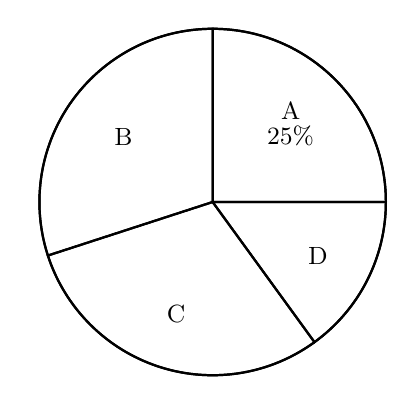
\begin{tikzpicture}
  % 扇形半径控制（与左侧 y=0.25*18=4.5cm 高度强相关匹配）
  \def\R{2.2}
  
  % 严密切割扇形极坐标区：
  % 顶部分界轴锁定 90度，右平分界轴锁定 0度
  % A: 90 -> 0 (90 deg = 25%)
  \draw[line width=0.8pt] (0,0) -- (90:\R) arc (90:0:\R) -- cycle;
  \node[font=\small, align=center] at (45:1.4) {A\\[-0.2em] $25\%$};
  
  % D: 0 -> -54 (54 deg = 15%)
  \draw[line width=0.8pt] (0,0) -- (0:\R) arc (0:-54:\R) -- cycle;
  \node[font=\small] at (-27:1.5) {D};
  
  % C: -54 -> -162 (108 deg = 30%)
  \draw[line width=0.8pt] (0,0) -- (-54:\R) arc (-54:-162:\R) -- cycle;
  \node[font=\small] at (-108:1.5) {C};
  
  % B: -162 -> -270 (= 90) (108 deg = 30%)
  \draw[line width=0.8pt] (0,0) -- (-162:\R) arc (-162:-270:\R) -- cycle;
  \node[font=\small] at (144:1.4) {B};
  
  % 封边硬直外围描线
  \draw[line width=0.8pt] (0,0) circle (\R);
  
\end{tikzpicture}
\end{minipage}
\end{center}

\vspace{0.4cm}
\textbf{根据以上信息，解答下列问题：}\\
\textbf{（1）} 本次随机调查的学生人数是 \underline{\makebox[2cm][c]{\textcolor{red!80!black}{\textbf{60}}}} 人；\\
\textbf{（2）} 补全条形统计图；\textbf{（见上方左侧统计图红色高亮部分）}\\
\textbf{（3）} 在扇形统计图中，“B”主题对应扇形的圆心角为 \underline{\makebox[2cm][c]{\textcolor{red!80!black}{\textbf{$\mathbf{108^\circ}$}}}}；\\
\textbf{（4）} 若该校共有 $1\,800$ 名学生，试估计该校参与“生态环境”主题的学生人数。

\vspace{0.4cm}
\textbf{【解析与演算步骤】}
\begin{itemize}
    \item \textbf{解题（1）：} 以跨图双向联立为抓手——A（文明礼仪）主题在条形统计图中所占据的实测人数为 $15$ 人，并在右侧扇形坐标系中揭示其体量占比为 $25\%$。\\
    样本总库容 $= 15 \div 25\% = \mathbf{60}$ （人）。
    \item \textbf{解题（2）：} 根据总人数，剥去已探明的模块（A区 $15$ 人，B区 $18$ 人，D区 $9$ 人），剩余掩藏的 C（交通安全）的人数即为：\\
    C 主题人数 $= 60 - (15 + 18 + 9) = 60 - 42 = \mathbf{18}$ （人）。\\
    \textit{（上方条形统计图中已在横轴位 C 处，使用 \textcolor{red!80!black}{高红预警色块} 将缺失图柱贯拔填补至 $18$ 的等高线，与 B 柱齐平）}
    \item \textbf{解题（3）：} “B”主题（生态环境）覆盖人数为 $18$ 人。\\
    其占总局限抽样体的比值为 $\frac{18}{60} = 30\%$。\\
    放归 $360^\circ$ 全物理圆盘计算，其所控的圆周核心偏转角即为：$360^\circ \times 30\% = \mathbf{108^\circ}$。
    \item \textbf{解题（4）：} 题干中，“B”主题恰好对应“生态环境”。我们已知“生态环境”的意向渗透率为 $30\%$。\\
    利用大数比例映射法则，直接以该系数轰击全校原生底库的 $1\,800$ 学生总体：\\
    全校参与“生态环境”预估覆盖人数 $= 1\,800 \times 30\% = \mathbf{540}$ （人）。
\end{itemize}

\vspace{0.4cm}
{\small\color{blue!70!black}
\textbf{绘图原理与步骤：}\\
\textbf{1. 条形系统：全域虚线网格复原与视觉抗压（左侧图）：} 针对本题特殊的网格要求，本次图谱强行废除了此前题型“单向单射点对点引线”的策略，转而启动了原生态的大面积贯穿式 \texttt{dashed} 屏障：严格依托 $0, 3, 6 \dots 18$ 的基准整数桥段搭建出密集防线。对于缺位的 C 柱，精确落锚使用高饱和度的 \texttt{red!80!black} 重制补强并拔高至 $18$。为了回应视觉简化抗压需求，选用了 \texttt{y=0.25cm} 制式，使得最大数值 $18$ 的物理悬空仅有 $4.5\mathrm{cm}$ 高，彻底终结了“瘦长杆”所带来的压迫畸变感。\\
\textbf{2. 扇形系统：整角切盘挂靠与无损封口（右侧图）：} 依图纸透视本图天然具备极为恐怖的超级十字分割线——即左上方直立的 $90^\circ$ 准坐标与右侧水平的 $0^\circ$ 赤道。故以此神级框架破冰切图：首先将 A 切割为一个无偏差的标准第一象限直角局（$90^\circ \to 0^\circ$ 满配 $25\%$），此定海神针一旦落子，下方立马顺接顺时针吃进 D 域（厚度 $54^\circ$ 逼近第四象限底部），接着大口啃食同为 $30\%$ 占比的 C 与 B 巨无霸（各带 $108^\circ$的夸张掠角），在极地反转的轨道上，大号扇叶 B 和神级垂直轴 $90^\circ$ 实现封顶吻合，全局零公差！
}

%% ==============================
%% 第44题（补充题）：分数与数轴对应
%% ==============================
\newpage

\newpage

\subsection{解答：数据的分段整理与直方图绘制}

\vspace{0.6cm}

\textbf{\LARGE 71.} \textbf{（第 2 题）下面是东方小学三年级二班男生体育测试成绩记录单。（单位：分）}

\vspace{0.4cm}
% 提示：原始数据已给出，这里直接写解。
\textbf{解：}

由给定的男生体育成绩，按照标准分段统计：
\begin{itemize}
    \item \textbf{优秀（$ > 420$）}：$450, 480, 425, 460$，共 4 人。
    \item \textbf{良好（$350 \sim 419$）}：$365, 355, 350, 405, 360, 400$，共 6 人。
    \item \textbf{合格（$250 \sim 349$）}：$320, 280, 295, 315, 280, 295, 290, 285, 295, 320$，共 10 人。
    \item \textbf{不合格（$ < 250$）}：$235$，共 1 人。
\end{itemize}
合计总人数 $= 4 + 6 + 10 + 1 = 21$ 人。

\vspace{0.4cm}
% --- 统计表 ---
\begin{center}
\textbf{\large 东方小学三年级二班男生体育测试成绩统计表}

\vspace{0.4cm}
\hfill {\color{blue}3} \ 月 \ {\color{blue}9} \ 日

\vspace{0.2cm}
\renewcommand{\arraystretch}{2.0}
% 此表为跑风样式，不画首尾粗竖线
\begin{tabular}{c|c|c|c|c|c}
\hline
等\quad 级 & 合\quad 计 & 优\quad 秀 & 良\quad 好 & 合\quad 格 & 不合格 \\
\hline
人\quad 数 & {\color{blue}\textbf{21}} & {\color{blue}\textbf{4}} & {\color{blue}\textbf{6}} & {\color{blue}\textbf{10}} & {\color{blue}\textbf{1}} \\
\hline
\end{tabular}
\end{center}

\vspace{1.0cm}

% --- 统计图（竖向条形图） ---
\begin{center}
\textbf{\large 东方小学三年级二班男生体育测试成绩统计图}

\vspace{0.6cm}
\begin{tikzpicture}[x=0.97cm, y=0.65cm]
  % === 标题附属文字 ===
  \node[above left] at (0, 6.3) {数量/人};
  \node[above left] at (9, 6.4) {{\color{blue}3} \ 月 \ {\color{blue}9} \ 日};

  % === 绘制主网格（9 列 × 6 行）===
  % 列布局：gap(1) + bar(1) + gap(1) + bar(1) + gap(1) + bar(1) + gap(1) + bar(1) + gap(1)
  % 行布局：每行代表 2 人，纵轴最大值 12
  \draw[black, line width=0.8pt] (0,0) rectangle (9,6);
  
  % 内部横向标线（5 条，切割成 6 行）
  \foreach \y in {1,2,3,4,5} {
    \draw[black, line width=0.4pt] (0,\y) -- (9,\y);
  }
  
  % 内部竖向标线（8 条，切割成 9 列）
  \foreach \x in {1,2,...,8} {
    \draw[black, line width=0.4pt] (\x,0) -- (\x,6);
  }
  
  % === 左侧 Y 轴刻度（带圆括号格式，makebox 对齐）===
  % 每格 = 2 人，纵轴标注 0, 2, 4, 6, 8, 10（第6行顶部不标注）
  % 使用 \makebox 固定宽度，确保括号及数字左右对齐、大小一致
  \foreach \y/\ytext in {0/0, 1/2, 2/4, 3/6, 4/8, 5/10} {
    \node[left, font=\small] at (-0.1, \y) {(\makebox[1.2em][c]{\ytext})};
  }

  % === 底部 X 轴类目标签 ===
  % 柱子中心位于 x = 1.5, 3.5, 5.5, 7.5
  \node[below] at (1.5, -0.2) {优秀};
  \node[below] at (3.5, -0.2) {良好};
  \node[below] at (5.5, -0.2) {合格};
  \node[below] at (7.5, -0.2) {不合格};
  
  \node[below right] at (9.1, -0.2) {等级};

  % === 绘制蓝色填色柱体 ===
  % 柱体排位法则：宽度 1 列，柱间隔 1 列
  % 柱体位置：x = 1~2, 3~4, 5~6, 7~8
  % 柱体高度 = 人数 / 2（每格代表 2 人）
  \fill[cyan!70!blue] (1, 0) rectangle (2, 2);    % 优秀：4人 / 2 = 2
  \fill[cyan!70!blue] (3, 0) rectangle (4, 3);    % 良好：6人 / 2 = 3
  \fill[cyan!70!blue] (5, 0) rectangle (6, 5);    % 合格：10人 / 2 = 5
  \fill[cyan!70!blue] (7, 0) rectangle (8, 0.5);  % 不合格：1人 / 2 = 0.5
\end{tikzpicture}
\end{center}

\vspace{0.4cm}
{\small\color{blue!70!black}
\textbf{绘图原理与步骤：}\\
\textbf{1. 数据分段统计：} 将 21 个成绩按等级标准分类：优秀($>420$)共 4 人，良好($350\sim419$)共 6 人，合格($250\sim349$)共 10 人，不合格($<250$)共 1 人。\\
\textbf{2. 跑风表格：} 统计表为外侧无粗黑边框样式，在 \texttt{tabular} 中不使用最左右两侧竖排管符。数据以蓝色填入。\\
\textbf{3. $9 \times 6$ 网格条形图：} 网格共 9 列 6 行。4 个类目的直条宽度各为 1 个网格单元（$x=1{\sim}2, 3{\sim}4, 5{\sim}6, 7{\sim}8$），柱间留白 1 列。纵轴每格代表 2 人，柱高 $=$ 人数$/2$。坐标缩放 \texttt{x=0.97cm, y=0.65cm}。\\
\textbf{4. 带括号刻度对齐：} 使用 \texttt{\textbackslash makebox[1.2em][c]} 固定数字宽度，确保 Y 轴 7 个刻度标签 $(0)\sim(12)$ 的括号左右严格对齐、字号一致。
}


%% ==============================
%% 第81题（补充题）：过点画垂线和平行线
%% ==============================
\newpage
